\section{Problembeskrivelse}

\begin{tcolorbox}[
    colback=gray!10,
    colframe=gray!50,
    title=Problem/behov – krav fra oppgaveteksten
]
\textbf{Problem/behov}
\begin{itemize}
    \item Definer og beskriv problemet dere ønsker å løse. Hvem har problemet?
    Hvordan løses dette i dag? Hva er samfunnsmessige ringvirkninger av problemet?
    Hvor stort er problemet (f.eks.\ kan man si noe om hvor mange det berører)?
    Består problemet av flere delproblem?
    \item Basert på informasjon dere henter inn, lag et konsept for en teknologisk
    løsning som har et kommersielt potensial. Løsningen skal henge sammen med
    problemet dere tar utgangspunkt i. Løsningen trenger ikke å beskrives i detalj,
    men jo mer informasjon man har på plass jo enklere vil det være å gjøre
    beregninger senere.
    \item Vurder om problemet er økende sett i lys av samfunnsmessige og
    bærekraftsmessige utfordringer frem mot år 2030. Kan man si at konseptet deres
    støtter nødvendig omstilling for å løse disse utfordringene?
    \item Beskriv styrkene i gruppa som gjør dere godt egnet til å løse dette
    problemet og til å utvikle konseptet.
\end{itemize}
\end{tcolorbox}

\subsection{Problem og behov}

Norges jernbaneinfrastruktur er under betydelig press. Det norske jernbanenettet omfatter om lag 4\,000 kilometer bane, over 2\,700 broer samt et stort antall tunneler og fjellskjæringer \parencite{jernbanedirektoratet_tall}. Mange av disse konstruksjonene er av høy alder og utsatt for kontinuerlig slitasje fra klima, frost og geologiske bevegelser. Det akkumulerte vedlikeholdsetterslepet er estimert til 127,8 milliarder kroner \parencite{banenor_infrastatus_2024}, og til tross for at 437 milliarder kroner er avsatt til jernbaneformål i Nasjonal transportplan (NTP) 2025--2036, vurderer bransjeaktører at dette ikke er tilstrekkelig til å ta inn etterslepet i planperioden \parencite{jernbanedirektoratet_ntp_2025}.

Konsekvensene av utilstrekkelig vedlikehold er målbare. Feil på infrastrukturen sto for om lag 24 prosent av forsinkelsestimene og nærmere 44 prosent av innstilte persontog i andre tertial 2024 \parencite{jernbanedirektoratet_gjennomforingsplan_2025}. Sett over hele 2024 var om lag 34 prosent av persontogene forsinket eller innstilt \parencite{vg_tog_2025}, og Bane NORs punktlighetsmål på 90 prosent ble ikke nådd \parencite{banenor_punktlighet_2025}. Dette rammer arbeidspendlere, reisende og godstransport, og svekker tilliten til jernbanen som foretrukket transportmiddel.

\textit{Primærkundene} -- de som eier problemet -- er infrastrukturforvaltere med ansvar for drift og vedlikehold av jernbanen, i Norge særlig Bane NOR SF. Sekundært berøres togoperatørene (Vy, SJ, GoAhead m.fl.), som er avhengige av infrastrukturens tilstand for å levere punktlige avganger, og i siste instans passasjerene og samfunnet for øvrig.

\subsubsection{Dagens praksis og dens begrensninger}

Bane NOR opererer med to parallelle inspeksjonsspor for jernbanebroer: årlige driftskontroller med begrenset dokumentasjonskrav og grundige ingeniørkontroller hvert sjette år (\cref{kontakt:traetten}). Menneskebetjente droner brukes allerede til bildedokumentasjon ved ingeniørkontroller av broer og høye fjellskjæringer, men krever at en operatør transporteres til stedet for hver gjennomgang (\cref{kontakt:traetten}). For spormåling benyttes i tillegg målevognen Roger 1000 (\cref{kontakt:lau}). Den største operative utfordringen er sportilgang: strenge sikkerhetsregler krever togfrie perioder, som presser inspeksjoner til nattarbeid og begrenser hva som faktisk gjennomføres innenfor et år (\cref{kontakt:traetten}). Den viktigste svakheten i dagens regime er imidlertid ikke datainnsamlingen, men dataanalysen -- innsamlede data sammenlignes fortsatt i stor grad manuelt mot grenseverdier, uten systematisk utnyttelse av historiske trender (\cref{kontakt:lau}).

Problemet kan dekomponeres i tre delproblem:

\begin{enumerate}
    \item \textbf{Lav inspeksjonsfrekvens.} Inspeksjonsintervallet er fast, ikke tilstandsbasert, slik at tilstandsforringelse som oppstår mellom planlagte gjennomganger kan forbli uoppdaget. Eldre infrastruktur kan feile uten forvarsel (\cref{kontakt:traetten}).
    \item \textbf{Personellrisiko.} Manuell inspeksjon i og nær spor og på høye broer medfører HMS-risiko. Krav til sikkerhetsvakter begrenser i tillegg effektiv utnyttelse av tilgjengelig inspeksjonstid (\cref{kontakt:traetten}).
    \item \textbf{Reaktivt vedlikehold.} Mangel på kontinuerlige tilstandsdata og automatisert analyse gjør det vanskelig å drive prediktivt vedlikehold. AI-drevet analyse trekkes frem som det største enkeltforbedringspotesialet i dagens inspeksjonsregime (\cref{kontakt:lau}).
\end{enumerate}

\subsection{Teknologisk konsept}

Konseptet tar utgangspunkt i et konkret og dokumentert markedsbehov (\textit{market pull}), men muliggjøres av kommersielt tilgjengelig droneteknologi og moden AI-basert bildeanalyse som nå er klar for industriell anvendelse (\textit{technology push}). Kombinasjonen av disse to kreftene skaper et gunstig mulighetsvindu \parencite{torvatn_teknologiledelse_2024}.

Det foreslåtte konseptet er et autonomt dronesystem for kontinuerlig tilstandsovervåking av kritiske infrastrukturobjekter langs jernbanen -- tunneler, broer og fjellskjæringer. Systemet består av autonome droner stasjonert i dedikerte dokkingstasjoner plassert permanent ved utvalgte objekter. Dronene utfører forhåndsdefinerte eller hendelsesstyrte inspeksjonsruter -- for eksempel etter kraftig nedbør, frostperioder eller registrerte trafikkavvik -- og samler inn bilde- og sensordata som analyseres over tid for å avdekke gradvise endringer i konstruksjonenes tilstand. En konseptuell illustrasjon av systemet i operasjon er vist i \cref{fig:drone_concept}, mens den overordnede systemarkitekturen er vist i \cref{fig:system_overview}.

\begin{figure}[ht]
    \centering
    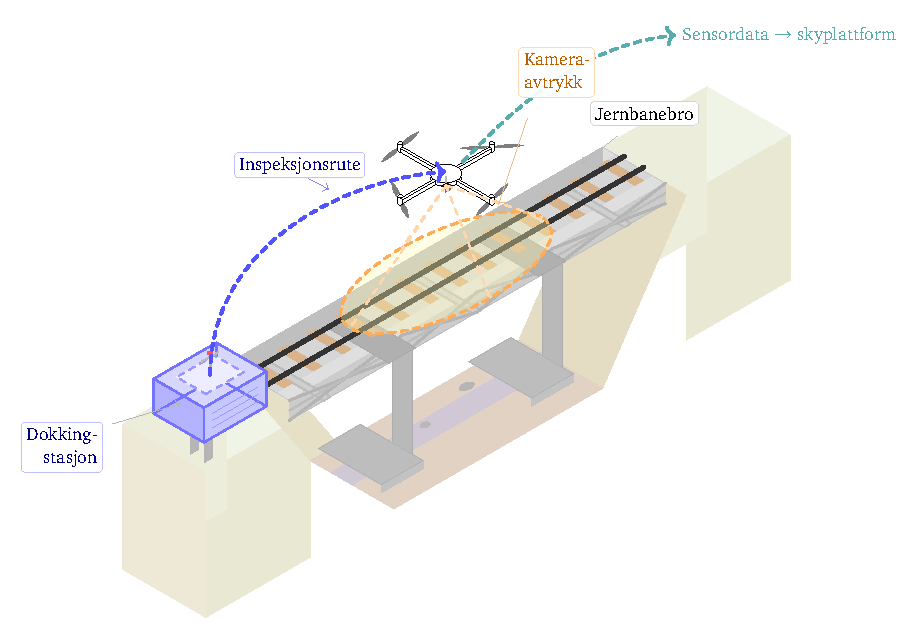
\includegraphics[width=\textwidth]{figurer/drone_figure.pdf}
    \caption{Konseptuell illustrasjon av det autonome dronesystemet i operasjon over en jernbanebro. Dronen letter fra sin permanente dokkingstasjon, følger en forhåndsdefinert inspeksjonsrute og samler inn bilde- og sensordata (oransje kameraavtrykk) som overføres til en skyplattform for analyse.}
    \label{fig:drone_concept}
\end{figure}

\begin{figure}[ht]
    \centering
    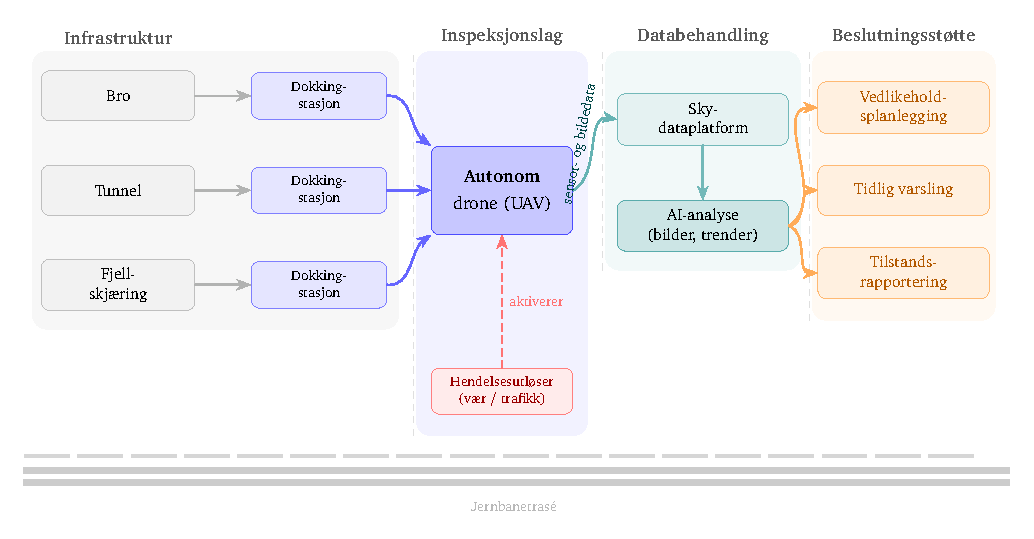
\includegraphics[width=\textwidth]{figurer/system_overview.pdf}
    \caption{Overordnet systemarkitektur. Broer, tunneler og fjellskjæringer utstyres med permanente dokkingstasjoner hvorfra autonome droner utfører planlagte eller hendelsesstyrte inspeksjoner. Innsamlede data overføres til en skybasert plattform for AI-analyse og genererer beslutningsstøtte i form av vedlikeholdsplanlegging, tidlig varsling og tilstandsrapportering.}
    \label{fig:system_overview}
\end{figure}

Konseptet har tydelige paralleller til pågående initiativ internasjonalt. I Spania har luftfartsmyndigheten AESA gitt selskapet Ineco tillatelse til å benytte autonome droner i dokkingstasjoner til jernbaneinspeksjon \parencite{railwaygazette_spain_2024}. Den internasjonale jernbaneunionen (UIC) driver prosjektet Drone4Rail, som i samarbeid med EASA utvikler et regulatorisk rammeverk for langdistanse BVLOS-inspeksjon av jernbane \parencite{uic_drone4rail_2024}. EU-prosjektet RADIUS (Railway Digitalisation Using Drones) har videre utarbeidet konsepter for droneintegrerte dokkingstasjoner og trafikkstyring \parencite{euspa_radius_2024}. I Norden gjennomførte EU-prosjektet Drones4Safety verdens første vellykkede landing og lading av en autonom drone på en høyspentlinje, demonstrert ved Aarhus Letbane i 2022. Prosjektet estimerer et besparelsespotensial på €15 mrd. årlig for europeisk transportinfrastruktur ved full kommersialisering (\cref{kontakt:ebeid}).

Også i Norge er behovet empirisk bekreftet. Bane NOR omtaler automatisert tilstandsovervåking internt som «vegen videre for jernbanen», og et konkret prosjekt med autonom dronestasjon på Meråkerbanen i Trøndelag er planlagt igangsatt 2026--2027 med midler allerede bevilget (\cref{kontakt:traetten}). Nordic Unmanned, en norsk droneoperatør, drifter allerede syv permanente drone-i-boks-systemer for kritisk infrastruktur i Belgia og Finnmark og gjennomførte om lag 2\,500 flyvninger i 2025 (\cref{kontakt:wike}). Disse initiativene bekrefter at det teknologiske og regulatoriske grunnlaget for konseptet er i ferd med å modnes, og at norsk jernbane er godt posisjonert for tidlig adopsjon.

Innovasjonsmessig er konseptet primært en \textit{inkrementell innovasjon}: droner og jernbaneinspeksjon eksisterer begge som separate fenomener, og løsningen kombinerer disse på en ny måte. Konseptet har likevel et element av \textit{disruptiv innovasjon} ved at det retter seg mot et kundesegment -- behovet for kontinuerlig, hendelsesstyrt tilstandsovervåking -- som dagens aktører ikke betjener \parencite[]{torvatn_teknologiledelse_2024}.

Konseptets verdiforslag kan formuleres slik: [PRODUKTNAVN] hjelper infrastrukturforvaltere som Bane NOR, som i dag mangler kontinuerlig og kostnadseffektiv tilstandsovervåking av kritiske jernbanestrukturer, til å gå fra reaktivt til prediktivt vedlikehold -- uten at inspeksjonspersonell trenger å oppholde seg i spor eller på høye konstruksjoner.

\subsection{Problemets utvikling mot 2030}

Problemet må vurderes som \textit{voksende} frem mot 2030, av tre grunner. For det første eldes jernbaneinfrastrukturen raskere enn den fornyes, slik at vedlikeholdsetterslepet øker år for år. For det andre er klimaendringene forventet å øke hyppigheten av ekstreme værhendelser som kraftig nedbør, flom og ras -- hendelser som direkte truer jernbaneinfrastruktur og øker behovet for hyppig tilstandsovervåking. For det tredje skaper den politiske satsingen på jernbane som ryggraden i et bærekraftig transportsystem -- slik det fremgår av NTP 2025--2036 \parencite{jernbanedirektoratet_ntp_2025} -- et økt behov for pålitelig og kostnadseffektiv forvaltning av eksisterende infrastruktur. Den dypere bærekraftsmessige analysen av konseptet, herunder livsløpsvurdering og kobling til FNs bærekraftsmål, behandles i \cref{sec:miljoanalyse}.

\subsection{Gruppens styrker og kompetanse}

Prosjektgruppen består av fem tredjårsstudenter i ingeniørutdanning ved NTNU: to med fordypning i elektroingeniørfag og tre i dataingeniørfag. Den tverrfaglige sammensetningen dekker sentrale deler av det foreslåtte systemet -- sensorteknologi og signalbehandling på den ene siden, og programmering, maskinlæring, datalagring og systemutvikling på den andre -- og gir gruppen et solid teknisk grunnlag for å analysere og videreutvikle konseptet.

Gjennom faglige og personlige nettverk har gruppen tilgang til kontakter med erfaring fra kollektivtransport og jernbanerelatert virksomhet, blant annet fra Sporveien og NTNU-miljøet rundt jernbane og autonome systemer. Dette åpner for kvalitative intervjuer med fagpersoner som besitter innsikt i operative utfordringer, sikkerhetskrav og praktiske rammebetingelser for inspeksjon og vedlikehold -- noe som vil styrke det empiriske grunnlaget for prosjektet.

Gruppen er bevisst på at videre kommersialisering vil kreve kompetanse som gruppen foreløpig ikke besitter: primært innen flysertifisering og BVLOS-regulering, jernbanespesifikke HMS-krav og kommersiell anskaffelsesprosess mot offentlig sektor. For å dekke disse kompetansegapene vil gruppen arbeide systematisk med å identifisere samarbeidspartnere, herunder norske droneselskaper med erfaring fra BVLOS-operasjoner, juridiske rådgivere innen luftfartsrett og eventuelle industripartnere med erfaring fra Bane NOR-prosjekter. En slik partnerstruktur er i tråd med anbefalinger fra faglitteraturen om at teknologioppstartsselskaper bør kompensere for manglende bransjekunnskap gjennom strategiske allianser \parencite[84]{torvatn_teknologiledelse_2024}.

\subsection{Grunnhypoteser}

I tråd med \textcite[57]{torvatn_teknologiledelse_2024} etableres følgende
grunnhypoteser som utgangspunkt for mulighetsstudiet:

\begin{enumerate}
    \item \textbf{Problem--løsning.} Produktet/tjenesten løser problemet med manglende kontinuerlig, kostnadseffektiv og sikker tilstandsovervåking av kritisk jernbaneinfrastruktur ved å tilby autonome, permanent stasjonerte droneinstallasjoner som utfører hendelsesstyrte inspeksjoner uten direkte menneskelig involvering.

    \item \textbf{Kunde.} Primærkunden er infrastrukturforvaltere med ansvar for drift og vedlikehold av jernbane -- i første omgang Bane NOR SF i det norske markedet, med potensial for skalering til øvrige europeiske jernbaneforvaltere.

    \item \textbf{Betalingsvilje.} Kunden vil kjøpe løsningen fordi den reduserer kostnader knyttet til reaktivt vedlikehold og driftsavbrudd, forbedrer HMS for inspeksjonspersonell og gir et bedre og mer kontinuerlig beslutningsgrunnlag for prioritering av vedlikeholdstiltak. Betalingsvilje er empirisk bekreftet: Bane NOR har allerede bevilget midler til et droneovervåkingsprosjekt på Meråkerbanen (\cref{kontakt:traetten}), og ifølge Albert Lau ved NTNU er slik vilje til stede i bransjen, men forutsetter dokumentert effekt -- gjerne med referanser fra andre europeiske land (\cref{kontakt:lau}).

    \item \textbf{Differensiering.} Løsningen skiller seg fra dagens operatørstyrte droner ved å være permanent stasjonert ved spesifikke kritiske objekter og ved å kombinere hendelsesstyrt inspeksjon med longitudinell dataanalyse. Dette muliggjør tidlig varsling og prediktivt vedlikehold -- noe dagens periodiske, transportbaserte inspeksjonsmetoder ikke kan tilby.

    \item \textbf{Markedsvindu.} Det er en unik mulighet i markedet fordi jernbanesektoren globalt er midt i en digitaliseringsbølge, det europeiske regulatoriske rammeverket for BVLOS-operasjoner er i ferd med å modnes, og norsk jernbane har et akutt og erkjent behov for mer effektiv infrastrukturforvaltning -- kombinert med politisk prioritering av vedlikehold i NTP 2025--2036. Ifølge Albert Lau ved NTNU er de organisatoriske og regulatoriske barrierene større enn de tekniske (\cref{kontakt:lau}), noe som gir et fortrinn for aktører som posisjonerer seg tidlig i samarbeid med Bane NOR.
\end{enumerate}

Som et innledende rammeverk for de videre analysene presenteres i \cref{tab:pestel} en PESTEL-analyse av konseptet.

\begin{table}[ht]
    \centering
    \begin{tabular}{p{2cm}p{5cm}p{5cm}}
        \toprule
        \textbf{Forhold} & \textbf{Positive faktorer} & \textbf{Negative faktorer} \\
        \midrule
        Politiske &
        NTP 2025--2036 prioriterer vedlikehold og fornying av jernbane;
        regjeringens satsing på digitalisering og grønn transport &
        Offentlige anskaffelsesprosesser er langsomme og ressurskrevende;
        regulatorisk kompleksitet knyttet til BVLOS-godkjenning fra
        Luftfartstilsynet \\
        \addlinespace
        Økonomiske &
        Vedlikeholdsetterslep på 127,8 mrd.\ kr skaper stort marked;
        dronemarkedet for jernbaneinspeksjon vokser med 24\,\% CAGR mot
        2030; tjenestemodell (drone-as-a-service) senker terskelen for
        kundene &
        Høye initielle investeringskostnader for utvikling og installasjon;
        budsjettkutt i offentlig sektor kan forsinke anskaffelser \\
        \addlinespace
        Sosiale &
        Økt sikkerhet for inspeksjonspersonell ved å redusere arbeid i og
        nær spor; bedre regularitet styrker tilliten til jernbanen som
        samferdselsmiddel &
        Potensiell motstand mot automatisering fra fagforeninger og
        eksisterende inspeksjonspersonell \\
        \addlinespace
        Teknologiske &
        Moden og kommersielt tilgjengelig droneteknologi; fremskritt innen
        AI-basert bildeanalyse og BVLOS-kommunikasjon; EU-prosjekter
        (RADIUS, Drone4Rail) bygger regulatorisk og teknisk grunnlag &
        Krav om høy driftspålitelighet i krevende nordiske klimaforhold
        (kulde, fukt, is); begrenset batterilevetid; utfordringer med
        GPS-ytelse i og rundt tunneler \\
        \addlinespace
        Miljømessige &
        Erstatter fossildrevne inspeksjonskjøretøy;
        muliggjør tilstandsbasert vedlikehold som reduserer overforbruk
        av materialer; støtter klimatilpasning av infrastruktur &
        Produksjon og avfallshåndtering av litium-batterier og
        dronekomponenter har et miljøfotavtrykk \\
        \addlinespace
        Legale &
        EASA-harmonisering av droneregler i Europa åpner for skalering
        på tvers av landegrenser; standardscenarier (STS) forenkler
        driftsgodkjenning for kvalifiserte operatører &
        BVLOS-operasjoner krever individuell driftstillatelse fra
        Luftfartstilsynet med SORA-risikovurdering; usikkerhet rundt
        ansvar ved uønskede hendelser med autonome systemer \\
        \bottomrule
    \end{tabular}
    \caption{PESTEL-analyse for konseptet med autonome dronesystemer til
    jernbaneinspeksjon.}
    \label{tab:pestel}
\end{table}